\documentclass[../main.tex]{subfiles}
\graphicspath{{\subfix{../imgs/}}}
\begin{document}
\newpage

\chapter{Prior Work}

\section{Music Generation via Deep Learning}

\subsection{\textit{ImprovRNN} and \textit{GrooveVAE} by Magenta}

TODO: Complete this section


\subsection{\textit{Learning Expressive Musical Performance} - LSTMs/RNNs for musical generation}

In this paper, Oore et.al\cite{oore:1} propose a novel approach to music generation, concentrating on direct performance generation. This involves jointly predicting the notes and their expressive attributes, such as timing and dynamics, rather than just creating or interpreting scores. This is in direct contrast to models like ImprovRNN or GrooveVAE that separate the generation of musical phrases from their expressive attributes. Specific to this task, the authors emphasizes the importance of using a dataset that is appropriate for the task of generating expressive musical performances. This implies the need for a dataset that captures not just the notes but also the nuances of timing and dynamics. To satisfy this requirement, the authors turn to the International E-Piano Dataset, which contains midi-recorded performances of piano works on a Disklavier, capturing musical notes as well as their expressive information with very high fidelity

The model employed is an LSTM-based network with three layers, each consisting of 512 cells. The network uses a temporally non-uniform representation of data, with a vocabulary of 413 different events, including NOTE-ON, NOTE-OFF, TIME-SHIFT, and VELOCITY events. The TIME-SHIFT events are particularly notable for allowing the model to capture expressive timing. They enable the network to move the time step forward by increments of 8 ms up to 1 second, thus maintaining expressiveness in note timings.
The network operates on one-hot encoding over this event vocabulary, with each input to the RNN being a single one-hot 413-dimensional vector.

TODO: INCLUDE IMAGES FROM PAPER

The system was found to be effective in generating MIDI performances with expressive timing and dynamics. The feedback from professional composers and musicians suggested that the system's output resembled human performances in terms of local structure, like phrasing and dynamics, although it lacked long-term structural coherence. The conclusion highlights that the system sounds like a skilled pianist but lacks a clear long-term compositional plan, creating performances that are expressive but somewhat random in nature. This research marked a significant step in the field of generative music, especially in its focus on the expressiveness of musical performances. The use of LSTM networks for this purpose shows promising results in capturing the nuances that make music feel more human and less mechanically generated.

\subsection{\textit{Generating Music with Long-Term Structure} - A modified Transformer Architecture for Music Generation}

TODO: Complete this section

\section{Systems geared toward Musical Improvisation}

\subsection{\textit{Voyager} — George E. Lewis}

Voyager is a ``non-hierarchical, interactive musical environment that privileges improvisation" \cite{Lewis:1}. In this environment, an improvisor engages in dialogue with a computer-driven interactive virtual improvising orchestra. The program analyzes the human improvisers performance and uses the analysis to guide a complex, improvised response to the player, as well as an independent response from its own creative internal process

Voyager was conceived as a set of 64 asynchronously operating single-voice MIDI-controlled players, each of whom responds to and generates music in real-time. First, a low-level routine parses incoming MIDI data into separate streams, accommodating up to two human improvisers. The improvisers are either playing MIDI-equipped keyboard instruments or playing acoustic instruments that are interfaced with pitch detection devices that parse the sounds of acoustic instruments into MIDI data streams. A mid-level smoothing routine is also called to construct averages of pitch, velocity, probability of note activation, and note spacing.

In response, a global subroutine called \textit{setPhraseBehaviour}\ref{fig:voyager_setphrasebehaviour} (called in intervals of 5 - 7 seconds), continuously recombines the MIDI players into new ensemble combinations with defined behaviors. These behaviors define how players are in the new ensemble, choosing whether to let the new ensemble play alongside the older ensemble or to shut off the older ensemble entirely. Lewis created several varying sonic behavior groupings — some of which clash — such that they may be active simultaneously, or move in and out of a unified metric pulse. The \textit{setPhraseBehaviour} routine also includes its own subroutines that determine the choice of timbre, melody generation algorithm, pitch sets, volume range, transposition, tempo, note spacing, probability of playing a note, interval width range, MIDI-related ornamentation (Eg. reverb) and how these parameters may change over time. 

\begin{figure}[htbp]
    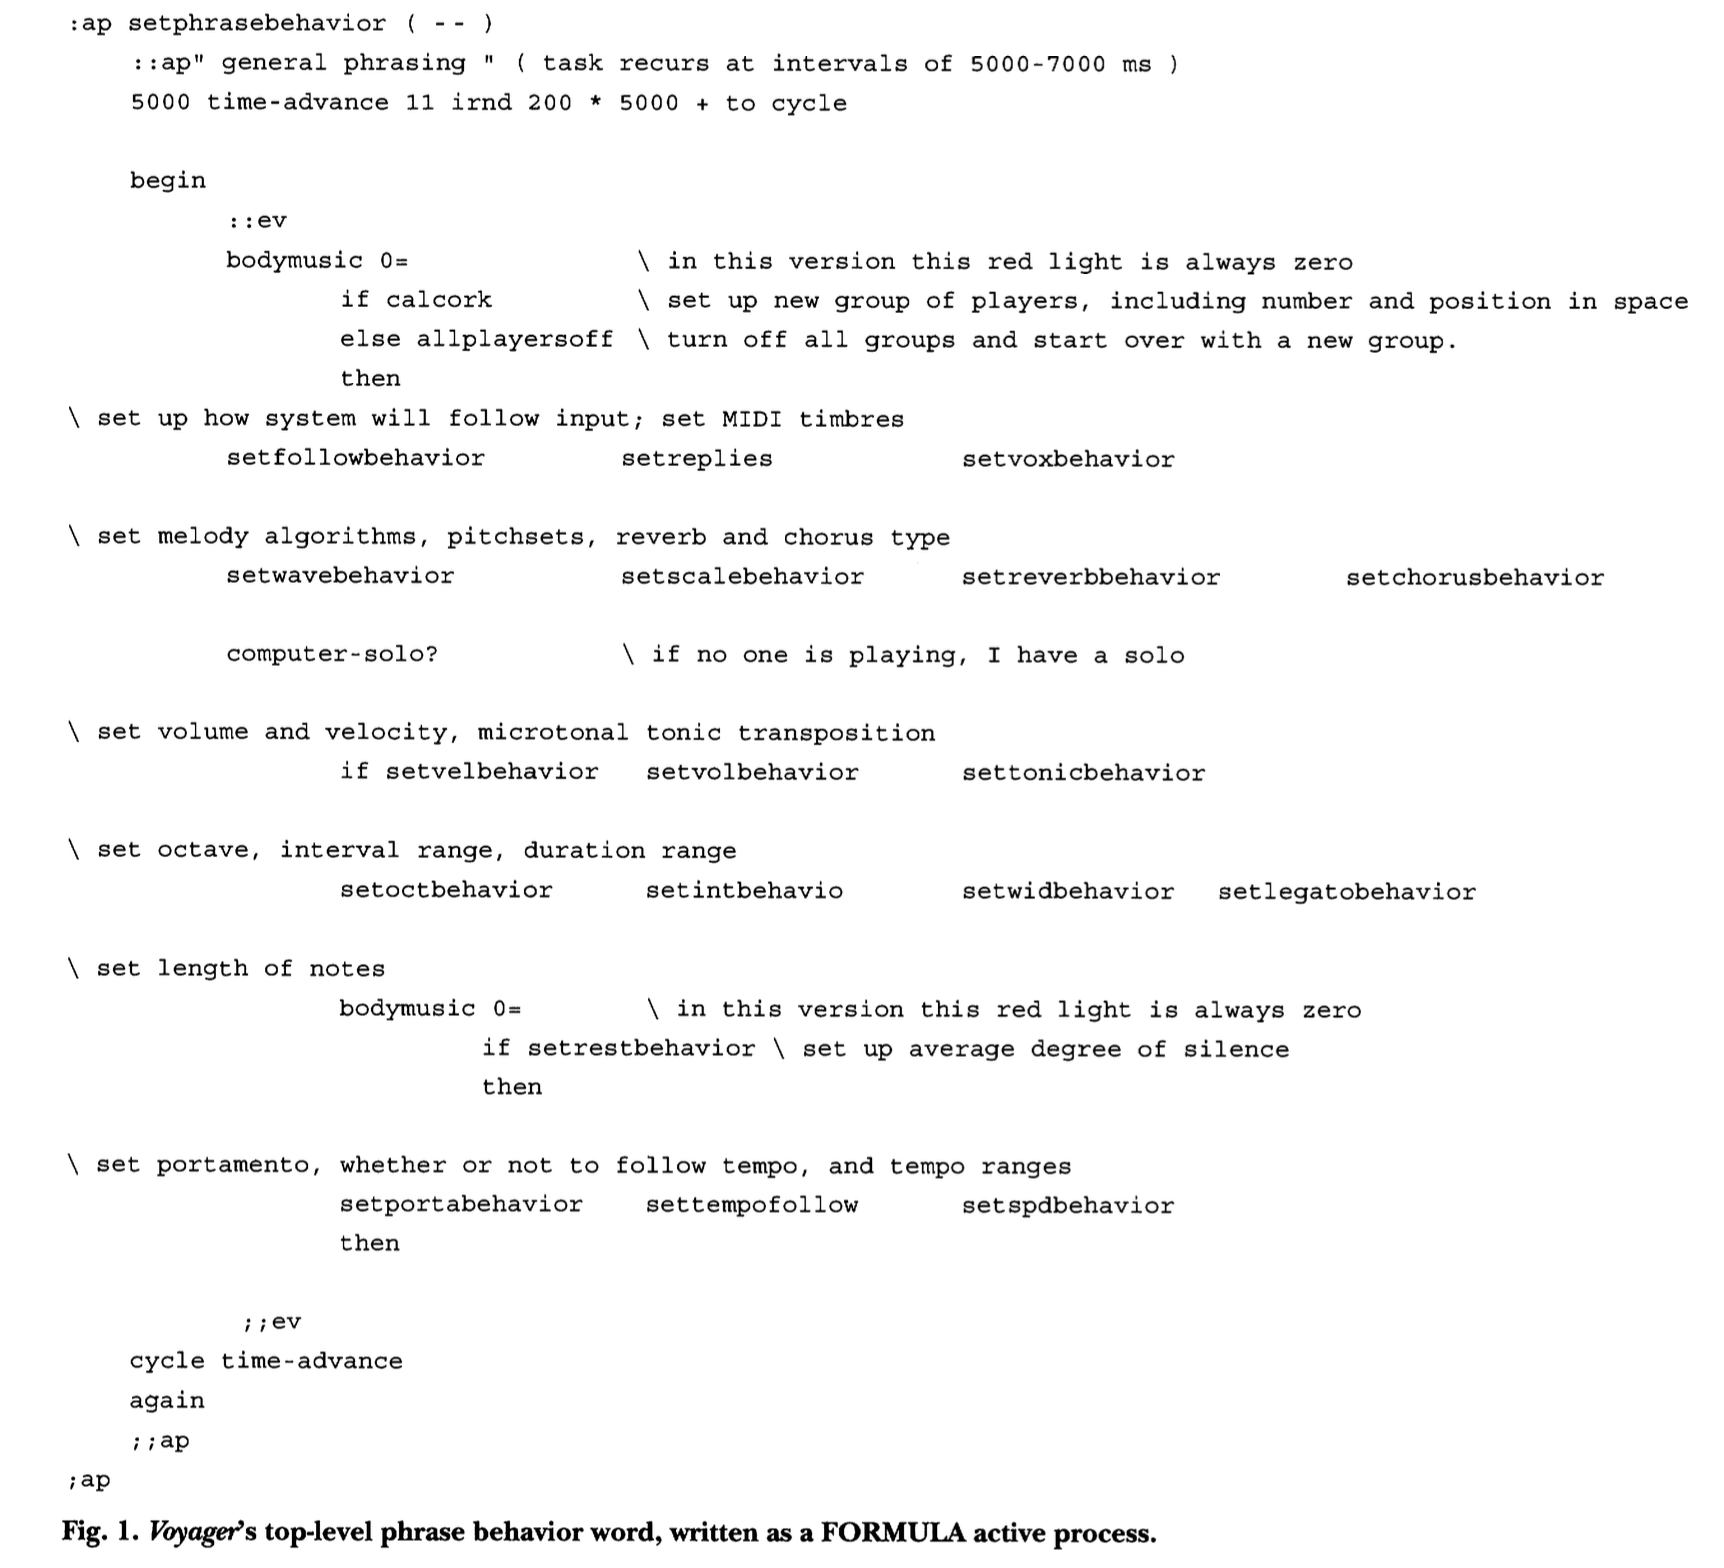
\includegraphics[width=1\textwidth,]{imgs/voyager_setphrasebehaviour.png}
    \caption{Voyager's setPhraseBehaviour Routine}
    \label{fig:voyager_setphrasebehaviour}
\end{figure}

Furthermore, each newly created ensemble chooses both a distinct group sonority, as well as a unique response to the input, deciding which improvisers — one, both, or none — influence its output behavior. The subroutine \textit{setresponse}\ref{fig:voyager_setresponse} runs asynchronously to \textit{setPhraseBehaviour}. This routine processes both the raw and the averages returned by the smoothing routine to decide how the ensemble responds to specific elements of the input, such as tempo, melodic intervals, etc. 

\begin{figure}[htbp]
    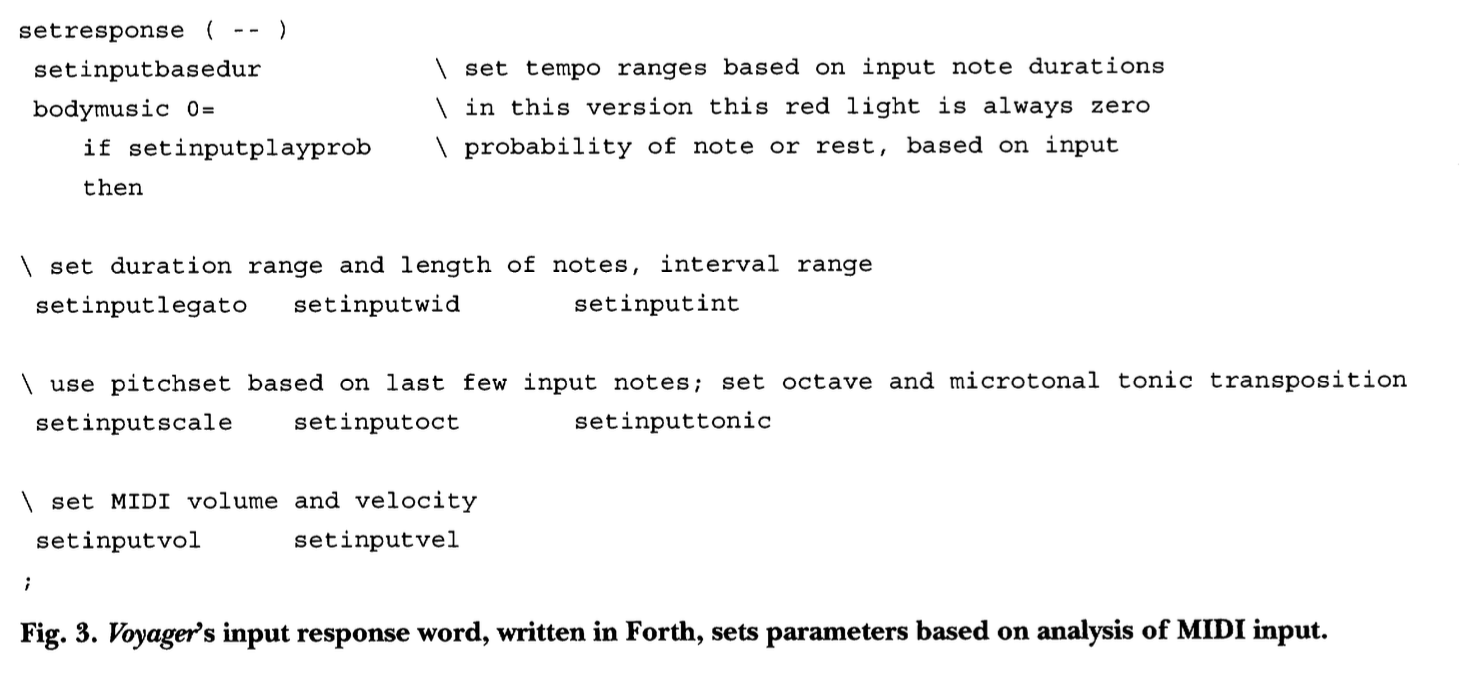
\includegraphics[width=1\textwidth,]{imgs/voyager_setresponse.png}
    \caption{Voyager's setResponse Routine}
    \label{fig:voyager_setresponse}
\end{figure}

A critical distinction between Voyager and other improvisatory systems is that Voyager is still able to function in the absence of any outside input. With no input, the specification of the system's behavior is entirely governed by \textit{setPhraseBehaviour}. Given that the computer is able to spontaneously create music that is in no way influenced by the improviser, decisions made by Voyager have consequences that must be accounted for by the listening improviser, creating a situation where both the computer and the improviser are held equally accountable for the final output. This is an especially desirable quality for an improviser program, and something worth replicating within our proposed Transformer model.

\subsection{\textit{GenJam} by John A. Biles}
GenJam\cite{Biles:1}, created by John A. Biles, is an interactive genetic algorithm that models a jazz improviser and performs as a featured soloist in the author’s Virtual Quintet. Previous papers published by Biles have described GenJam's hierarchically related populations of melodic ideas, its chromosome representations for those ideas, its genetic operators for evolving new ideas, and the training of new soloists. This training is done under the guidance of a human mentor, who listens to GenJam improvise and indicates "good" or "bad" accordingly, as a kind of reinforcement loop. The mentor's feedback is used to increment or decrement the fitness of individual melodic ideas and serves as the environment in which musical ideas persist, or are removed from the stored hierarchy. New ideas evolve by 1) selecting the “better” ideas to be parents 2) breeding “children” ideas using single-point crossover and musically meaningful mutation, and 3) replacing the “worse” ideas in the population with these new children.

In their paper, Biles demonstrates how a four-bar phrase is mapped into ``GenJam Normal Form (GJNF)'' and discusses the various mutation operators available to GenJam to create a musical response. A key strength of GenJam is that it was later optimized to "trade-fours" with the player in a very traditional jazz style \cite{Biles:2}. Many other improvising systems are unable to tell when a phrase ends (a massively subjective art in and of itself) which means they frequently interrupt another improvisor mid-phrase. GenJam instead hardcodes the knowledge of the four-bar phrase, removing the problem entirely. The high-level algorithm it uses to accomplish this is described below:

\begin{enumerate}
    \item GenJam first receives a chord progression for a specific tune, (read in from a data file) and constructs a chord-scale mapping for the entire tune. The table below provides an example of a chord scale-mapping used during the listening phase and in the playing phase of Jerome Kern's \textit{All the Things You Are}

    \begin{figure}[htbp]
        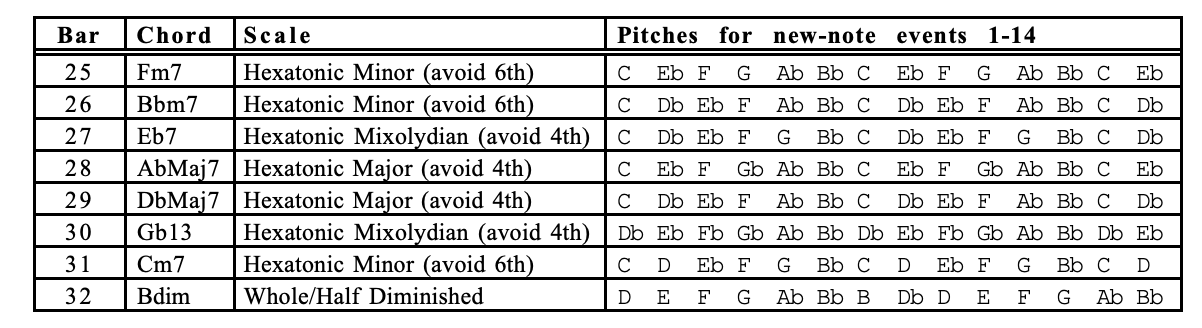
\includegraphics[width=1\textwidth,]{imgs/genJam_chordscalemapping.png}
        \caption{An Example of chord-scale mappings for the tune \textit{All the Things you are}, bars 25-32}
        \label{fig:genJam_chordscalemapping}
    \end{figure}
    
    \item The human performer plays four bars into a microphone plugged into a pitch-to-midi converter

    \begin{figure}[htbp]
        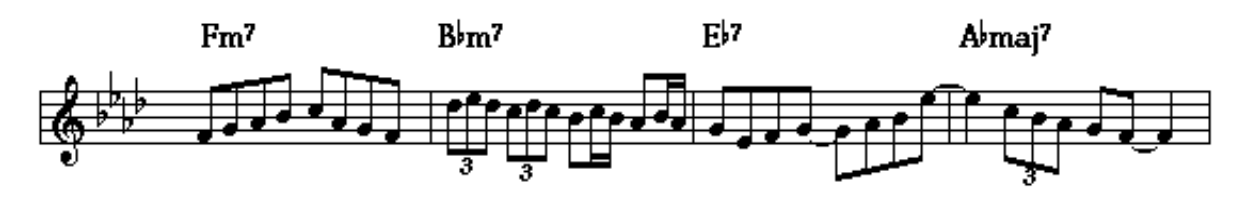
\includegraphics[width=1\textwidth,]{imgs/genJam_originaltune.png}
        \caption{An example of a Charlie Parker quote played over measures 25-28 of \textit{All the Things you are}}
        \label{fig:genJam_originaltune}
    \end{figure}

    \item The pitch to MIDI converter sends MIDI events to GenJam running on the host computer

    \item GenJam listens to MIDI events and quantizes them into 8th-note long windows. It then uses the chord-scale mappings provided to create measure and phrase chromosomes for the four-bar phrase in ``GenJam Normal Form (GJNF)''

    \begin{figure}[htbp]
        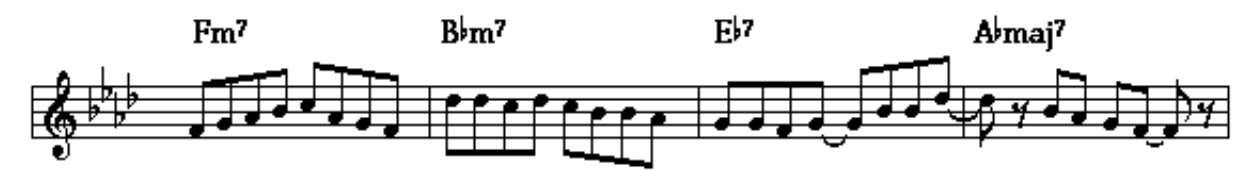
\includegraphics[width=1\textwidth,]{imgs/genJam_GJNFtune.png}
        \caption{The melody from figure \ref{fig:genJam_originaltune} in ``GenJam Normal Form''. Note that the triplet melodies cannot be preserved due to 8th note quantization}
        \label{fig:genJam_GJNFtune}
    \end{figure}

    \item In the last 30 milliseconds of the human’s four bar phrase, GenJam stops listening and performs musically meaningful mutations on some of the chromosomes in preparation to play them back as its next four. Since all the input has been converted to GJNF, the phrase may be mutated by using any of GenJam's musically meaningful mutation operators, which guarantees that the result is playable over the subsequent four-bar phrase. These mutations include reversing or inverting phrases, transposing phrases, repeating a phrase, and many other changes that can be combined to derive entirely new and musical four-bar phrases.

    \item Mutated chromosomes are then used as GenJam's next four bars as if they were part of a stored soloist

     \begin{figure}[htbp]
        \includegraphics[width=1\textwidth,]{imgs/genJam_mutatedTune.png}
        \caption{The four-bar phrase returned by GenJam to be played over bars 29-32}
        \label{fig:genJam_mutatedTune}
    \end{figure}
\end{enumerate}

The system of trading fours as presented here in GenJam is extremely robust. Compared to Voyager which functions largely in the space of free improvisation, GenJam makes full use of hard-coded information to make the performance work (eg. the data file with chord progressions for a specific tune). In our transformer model, it may be useful to include an interface that can hold similar information and essentially set the ``context" in which the improvised performance is happening.

\end{document}